\documentclass[11pt, twocolumn]{article}
\usepackage{titlesec}
\usepackage{tikz}
\usepackage{booktabs}
\usepackage{adjustbox} 
\usepackage{enumitem}
\usepackage{multirow}
\usepackage{bbding,enumitem}
\usepackage{authblk}
\usepackage{fancyhdr}
\usepackage{amsmath}
\usepackage{subcaption}
\usepackage[table]{xcolor}
\setcounter{secnumdepth}{3} % for adjusting padding
\pagestyle{fancy}
\newcommand{\blueoval}{%
    \begin{tikzpicture}[remember picture, overlay]
    \shade[shading=axis, left color=blue, right color=white] (current page.north west) -- (3,0) arc (0:180:4cm) -- cycle;
    \end{tikzpicture}%
}

\newcommand{\coloredfooter}{%
    \begin{tikzpicture}[remember picture, overlay]
    \shade[shading=axis, left color=teal, right color=white] (current page.south east) -- (-1,-2) arc (0:80:2cm) -- cycle;
    \end{tikzpicture}%
}

\fancyhf{} % Clear default header and footer
\fancyhead[L]{ \leftmark}
% Display section title in the left header
\fancyhead[R]{\thepage} % Display page number in the right header
\definecolor{mypink3}{cmyk}{0, 0.7808, 0.4429, 0.1412}

\makeatletter
\renewcommand{\maketitle}{\bgroup\setlength{\parindent}{0pt}
\begin{flushleft}
  \textbf{\@title}

  \@author
\end{flushleft}\egroup
}
\makeatother

\title{\Huge \color{mypink3}{ROV Document}  \vspace{0.5cm}}
\author{\Large E-JUST Robotics Club \normalsize \hspace{0.5cm} }

\setlength{\parindent}{0pt}
\date{\today}

\usepackage[showframe=false, margin=.75in]{geometry}

\usepackage{abstract}
\renewcommand{\abstractname}{}    % clear the title
\renewcommand{\absnamepos}{empty} % originally center

\usepackage{lipsum}

\usepackage{afterpage}

\renewenvironment{abstract}
 {\small
  \begin{center}
  \bfseries \abstractname\vspace{-.5em}\vspace{0pt}
  \end{center}
  \list{}{%
    \setlength{\leftmargin}{10mm}% <---------- Change margin here
    \setlength{\rightmargin}{\leftmargin}%
  }%
  \item\relax}
 {\endlist}

\usepackage[utf8]{inputenc}

%\usepackage{graphicx}
\usepackage{wrapfig}
\usepackage[lofdepth,lotdepth]{subfig}
\usepackage{booktabs}

\usepackage{rotating}

\usepackage{caption}
%\usepackage{subcaption}

%\usepackage[ngerman]{babel}

\usepackage{csquotes}

\setlength{\marginparwidth}{2cm} % Set marginparwidth to avoid todonotes issues
\usepackage{todonotes}

\usepackage{stfloats}

\usepackage[T1]{fontenc}
\usepackage{textcomp}
\usepackage{times}

\usepackage{framed} %um Boxen zu machen

\usepackage[citestyle=authoryear,
			bibstyle=authoryear,
			language=auto,
			url=false,
			backend=bibtex,
			doi=false,
			isbn=false]{biblatex}
	\renewbibmacro*{volume+number+eid}{%
  \printfield{volume}%
%  \setunit*{\adddot}% DELETED
  \setunit*{\addnbspace}% NEW (optional); there's also \addnbthinspace
  \printfield{number}%
  \setunit{\addcomma\space}%
  \printfield{eid}}
\DeclareFieldFormat[article]{number}{\mkbibparens{#1}}

\usepackage{setspace}
\onehalfspacing

\setlength{\columnsep}{0.8cm}

\setlength{\parskip}{0em}

\usepackage{color}
\definecolor{black}{gray}{0} % 10% gray

\usepackage[colorlinks=true,linkcolor=black,citecolor=black]{hyperref}

\usepackage{tabularx}
\newcolumntype{s}{>{\hsize=.5\hsize}X}

\usepackage{ntheorem}
\newtheorem*{TRQ}{Research Question}

\newtheorem{Hyp}{Hypothesis} 

\usepackage{graphicx}
\usepackage{fancyhdr}
\usepackage{lipsum}
\usepackage{geometry}
\usepackage{changepage} % To adjust page margins locally
\usepackage{afterpage}

% Apply the custom header and footer to all pages
\fancyfoot[L]{\hspace*{-1.9cm}{
\includegraphics[width=\paperwidth,height=1.9cm]{Images/Footer.png}}} % Footer

\pagestyle{fancy}
\makeatletter
\providecommand{\sf@counterlist}{} % Define sf@counterlist to avoid undefined control sequence
\makeatother

\usepackage{titlesec}

\titlespacing*{\subsection}{0pt}{5pt}{5pt}
\titlespacing*{\subsubsection}{0pt}{5pt}{5pt}

\setcounter{secnumdepth}{4}
\renewcommand\theparagraph{\thesubsubsection.\arabic{paragraph}}

\usepackage{tabularray}
\DefTblrTemplate{firsthead,middlehead,lasthead}{default}{}
\DefTblrTemplate{firstfoot}{default}{
  \UseTblrTemplate{contfoot}{default}
  \UseTblrTemplate{caption}{default}
}
\DefTblrTemplate{middlefoot}{default}{
  \UseTblrTemplate{contfoot}{default}
  \UseTblrTemplate{capcont}{default}
}
\DefTblrTemplate{lastfoot}{default}{
  \UseTblrTemplate{note}{default}
  \UseTblrTemplate{remark}{default}
  \UseTblrTemplate{capcont}{default}
}
\DefTblrTemplate{contfoot-text}{default}{Continue on the next column}
\DefTblrTemplate{capcont}{default}{\UseTblrTemplate{caption}{default}}
\UseTblrLibrary{booktabs}
\captionsetup{skip=3pt}
\SetTblrInner{rowsep=0pt, stretch=0.9}
\setlength{\headheight}{13.6pt}
\addtolength{\topmargin}{-1.6pt}
\setlength{\footskip}{58.2pt}

\begin{document}

\twocolumn

Fat Man float is inspired by the NSF-funded GO-BGC Project, which aims to build a global network of profiling floats to monitor ocean health. Similarly, our float is designed to perform multiple vertical profiles, diving from the surface to a depth of 2.5 meters, then returning to the surface. It records and transmits data, simulating real-world environmental monitoring devices.

\section{Mechanical Design}

The main float body (Figure \ref{fig:float}) is constructed from a transparent acrylic cylinder measuring 40 cm in length, 12 cm in outer diameter, and 3 mm in wall thickness. Acrylic was chosen for its ability to withstand hydrostatic pressure at a depth of 2.5 meters (approximately 25 kPa), its transparency which allows for visual inspection and early error detection, and its relatively low density of 1.19 g/cm³, offering better buoyancy characteristics compared to heavier materials like PVC or HDPE. Its specifications provide sufficient water displacement, maximizing buoyancy according to Archimedes' principle (Equation \ref{eq:archimedes})

\begin{equation}
\label{eq:archimedes}
    F_B = \rho_{\text{water}} \cdot g \cdot V_{\text{disp}}
\end{equation}

An HDPE disk, a material with a density close to water, is positioned to divide the cylinder into two sections. The upper section houses the electrical components, while the lower section serves as a water chamber for density control. The disk features grooves to mount O-rings, ensuring secure isolation between the two sections. 

\hspace{10pt} Additionally, chemical sealing agents such as epoxy are used to reinforce the isolation. The suction system uses two peristaltic pumps (Figure \ref{fig:pump}) for suction and ejection, operating at a flow rate of 60 ml/min, allowing the 700 ml chamber to be filled or emptied in approximately six minutes per operation. These pumps function by compressing a flexible tube with rotating rollers, generating a wave-like motion that pushes fluid through the tube, allowing precise flow control. To prevent leakage, the inlet and outlet hoses pass through PG-9 glands using 8 mm pneumatic hose. 

\begin{wrapfigure}{r}{0.4\columnwidth}
  \centering
  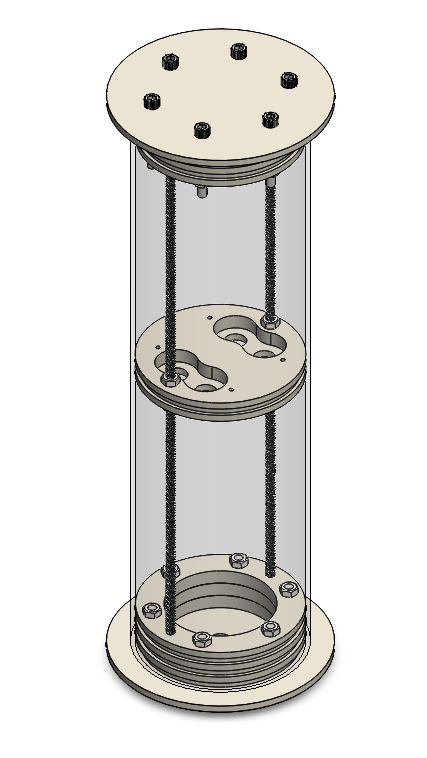
\includegraphics[width=0.39\columnwidth]{Images/Float.png}
  \caption{Illustrates the float mechanism, including 6mm lead screws, HDPE disk, and fastening nuts.}
  \label{fig:float}
\end{wrapfigure}

The float is sealed at both ends using custom end caps, each consisting of four stacked layers of HDPE. The outermost layer is 5 mm thick and exposed to water, while the remaining three layers are 10 mm thick and feature grooves designed to accommodate three O-rings for secure sealing. These layers are fastened together using bolts and nuts to ensure structural integrity and leak-proof performance. The end caps are friction-fit into the housing and are not secured with other fastening methods.

\begin{figure}[h]
  \centering
  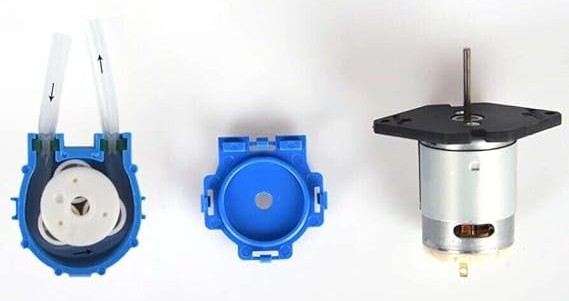
\includegraphics[width=\columnwidth]{Images/peristaltic pump.jpg}
  \caption{Illustrates the peristaltic pump inner parts and mechanism.}
  \label{fig:pump}
\end{figure}

\section{Electrical and Communication Systems}
\subsection{Main System}

The float's electrical system is designed on a single PCB (Figure \ref{fig:pcb}) to simplify maintenance and ensure reliable operation. This PCB integrates the STM32 microcontroller, a Real-Time Clock (RTC) module, an NRF24L01 radio module, a custom depth sensor (MS5837), an L298N motor drive, and multiple power converters to maintain stable performance.

\begin{figure}[h]
  \centering
  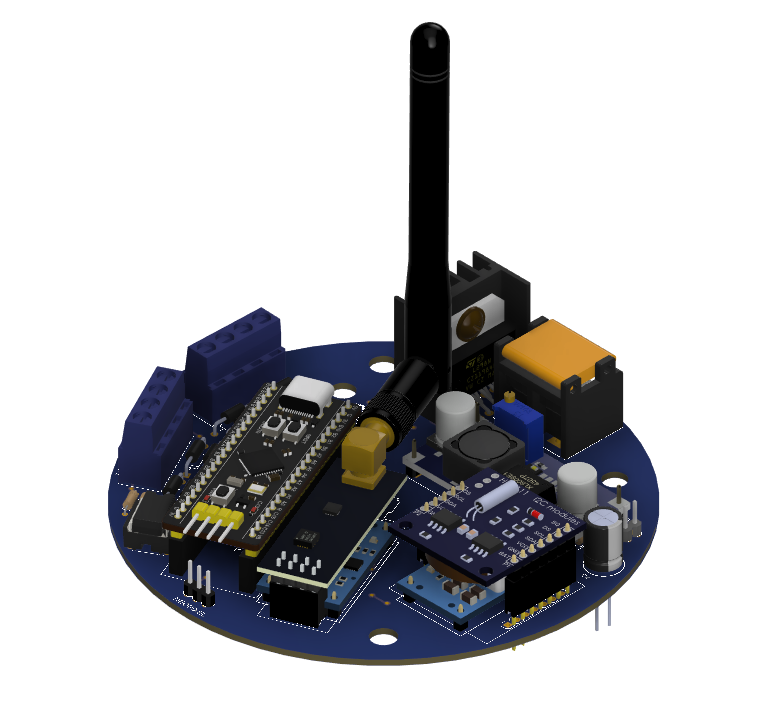
\includegraphics[width=\columnwidth]{Images/pcb.png}
  \caption{Fat Man's PCB design.}
  \label{fig:pcb}
\end{figure}

\hspace{10pt} The STM32 serves as the main controller, interfacing with the RTC, NRF24L01, MS5837 depth sensor, and L298N motor driver. It processes data from these components and transmits the collected information to the control station via a 2.4 GHz radio link.

\hspace{10pt} During vertical profiling, STM32 records sensor data at specific time increments while controlling the buoyancy engine to operate at equal intervals. The recorded data is stored along with the corresponding timestamps, ensuring accurate tracking of measurements throughout the profiling process. To accommodate the large volume of recorded data, an external EEPROM chip is connected to the STM32. The NRF24L01 radio module is responsible for transmitting all stored data to the control station, ensuring efficient data communication and retrieval.

\begin{table*}[b]
  \centering
  \begin{adjustbox}{max width=0.75\textwidth}
  \begin{tabular}{@{} l *{5}{c} @{}}
    \toprule
    \textbf{Component} & \textbf{Quantity} & \textbf{Voltage (V)} & \textbf{Current (A)} & \textbf{Power Per Unit (W)} & \textbf{Total Power (W)} \\
    \midrule
    NRF24L01            & 1 & 3.3   & 0.115     & 0.3795    & 0.3795   \\
    RTC Module                & 1 & 5   & 0.1   & 0.5    & 0.5   \\
    EEPROM           & 1 & 5    & 0.01      & 0.05     & 0.05     \\
    STM32 F411           & 1 & 5   & 0.25      & 0.25     & 0.25   \\
    Pumps/Motors	& 2	& 12	& 1	& 12	& 24 \\
    \midrule
   \multicolumn{5}{l}{\textbf{Total}} & \textbf{26.1795} \\
    \bottomrule
  \end{tabular}
  \end{adjustbox}
\caption{Power Calculation for the Non-ROV Device.}
\label{tab:power_calculation}
\end{table*}

\subsection{Battery Selection and Management}

To ensure a stable and reliable power supply, NiMH batteries were selected. The system consists of 20 NiMH cells. Ten cells are connected in series to provide a 12-volt output, and another set of 10 cells is connected in parallel with the first set. This configuration effectively increases both the current and capacity while maintaining the required voltage.

\hspace{10pt} The first 10 cells are divided into two packs, each containing 5 cells connected in a series. These two packs are then connected in series with each other to form the full 10-cell series configuration. This arrangement provides the necessary 12-volt output while ensuring efficient power delivery and stable operation.

\hspace{10pt} The entire system is charged using an external balance charger. This charger is responsible for balancing the voltage across the cells, ensuring uniform charging, preventing overcharging, and prolonging battery life.

\subsection{Fuse Calculations}

Total Power = 26.18W

Safety Factor = 1.5

Result = 3.2724375

Required Fuse: 5A

\end{document}